\documentclass[output=paper]{LSP/langsci} 
\author{Kunio Nishiyama\affiliation{Ibaraki University} 
}
\title{Phrasal compounds in Japanese} 
\abstract{Although Japanese does not have phrasal compounds analogous to English \textit{an} \textit{over the fence gossip} or \textit{a who’s the boss wink}, it does have phrasal compounds like \textit{kireena mati-dukuri}, literally ‘clean city-making,’ meaning construction of a clean city. This example illustrates one of several types of phrasal compounds in Japanese. The criteria that classify phrasal compounds in Japanese are 
(i) whether the head of the compound is a predicate, 
(ii) if a predicate, whether the head is of Sino-Japanese or of native origin, 
(iii) if not a predicate, whether the compound involves coordination or cliticization.

One source of phrasal compounding is noun incorporation. When an argument incorporates into a Sino-Japanese verbal noun predicate, we get what \citet{ShibataniKageyama1988} refer to as post-syntactic compounds, which have phrasal accent. In contrast, when an argument incorporates into a verbal noun predicate of native origin, we get a phrasal compound with word accent. The phrasal nature is evidenced by modifier stranding, and there are some conditions (e.g., pragmatic factors like cliché) on modifier stranding. There are three other sources of phrasal compounding which do not involve noun incorporation: natural coordination, enclitics, and proclitics. The first two have word accent and the last has phrasal accent. Whether a compound has word accent or phrasal accent is predicted by its structure: right branching compounds have phrasal accent (\citealt{Kubozono1995,Kubozono2005}). Kageyama’s (\citeyear{Kageyama1993,Kageyama2001,Kageyama2009}) notion of Word Plus is reconsidered and reclassified into three distinct classes: right-branching compounds, constructions involving proclitics, and phrases involving genitive deletion.}

\ChapterDOI{10.5281/zenodo.885125}
\maketitle

\begin{document}
\section{Introduction}\label{sec:nishiyama:1}
 
The term “phrasal compound” refers to compounds containing a phrase, in apparent violation of \citet{Botha1981} No Phrase Constraint, exemplified by the following \ili{English} examples:

\ea \label{ex:nishiyama:1} 
\ea  an over the fence gossip
\ex  a who’s the boss wink    \citep{Lieber1992}
\z
\z

Apparently parallel examples in \ili{Japanese} are as follows:

\ea\label{ex:nishiyama:2}
 \ea  
\gll Tokyo-kara-no nimotu\\
    Tokyo-from-\textsc{gen} package\\
\glt ‘a package from Tokyo’

  \ex 
\gll dare-ga    bosu-da-teki      taido\\
    who-\textsc{nom} boss-\textsc{cop}-like  attitude\\
\glt ‘a who’s the boss attitude’
\z
\z

In (\ref{ex:nishiyama:2}a), the \isi{genitive} \isi{marker} \textit{no} emerges between PP and the head noun. Thus, the example is not a compound but a phrase like its \ili{English} translation. In (\ref{ex:nishiyama:2}b), a morpheme -\textit{teki} ‘like’ attaches to the sentence ‘who’s the boss.’ The morpheme usually attaches to a word (e.g., \textit{hankoo-teki} ‘rebellion-like, rebellious’), but it has recently acquired the ability to attach to a phrase (the example in (\ref{ex:nishiyama:2}b) has an innovative or substandard flavor). The attachment of -\textit{teki} is a case of encliticization, which is discussed in \sectref{sec:nishiyama:4.2}. -\textit{teki} is also discussed in \sectref{sec:nishiyama:5}, but in the present context, it suffices to notice that (\ref{ex:nishiyama:2}b) as a whole is not a compound but a phrase like ‘a ”who’s the boss”-like attitude,’ consisting of a \isi{modifier} and the head noun. In short, neither of the examples in \REF{ex:nishiyama:2} is a compound. This is evidenced by the fact that (\ref{ex:nishiyama:2}a) and (\ref{ex:nishiyama:2}b) have \isi{phrasal accent}. Accent in \ili{Japanese} is described in §2.

Although the examples in \REF{ex:nishiyama:2} are not phrasal compounds, \ili{Japanese} does have phrasal compounds like the following:

\ea\label{ex:nishiyama:3}
\gll   kireena mati-dukuri  \\
    clean  {town making}\\
\glt ‘construction of a clean town’    \citep[518]{Kageyama2009}
\z

Here, \textit{mati-dukuri} is a compound, and \textit{kireena} modifies a part of the compound, resulting in a syntactic bracketing of [\textit{kireena mati}]\textit{-dukuri}. In other words, we have \isi{modifier} \isi{stranding}. This is a case of a bracketing paradox, for the bracketing in terms of \isi{phonological} words is [\textit{kireena}] \textit{mati-dukuri}. It is reminiscent of \textit{criminal lawyer}, with the meaning of a lawyer who practices criminal law (cf. \citealt{Beard1991}). With this meaning, the syntactic bracketing is [\textit{criminal}] \textit{law}]\textit{yer}. The difference is that \REF{ex:nishiyama:3} does not involve bound derivational morphemes but compounding.

The purpose of this paper is to describe and analyze phrasal compounds in \ili{Japanese}. Most of the examples discussed in this paper are reproduced from previous studies. However, in those previous studies, such examples of phrasal compounds are not discussed within an explicit perspective of phrasal compounds. This paper integrates several types of compounds within such a perspective. In addition to the type illustrated in \REF{ex:nishiyama:3}, \ili{Japanese} has a number of other types of phrasal compounds. The criteria used for classifying phrasal compounds in \ili{Japanese} are as follows: 
(i) Whether the head of the compound is a predicate; 
(ii) if the head is a predicate, whether it is of \ili{Sino-Japanese} origin (i.e. whether it is a vocabulary item in \ili{Japanese} which is of \ili{Chinese} origin), or whether it is of native origin; 
(iii) if the head of the compound is not a predicate, whether the compound involves coordination or cliticization.

This paper is organized as follows. \sectref{sec:nishiyama:2} briefly introduces accent in \ili{Japanese}, which is crucial in differentiating between words and phrases. In \sectref{sec:nishiyama:3}, phrasal compounds formed by noun \isi{incorporation} are discussed. There are two subtypes: one type involving \ili{Sino-Japanese} verbal nouns (3.1) and one type involving verbal nouns of native origin (\sectref{sec:nishiyama:3.2}). 
\sectref{sec:nishiyama:4} discusses phrasal compounds without noun \isi{incorporation}. There are three subtypes: one involving natural coordination (\sectref{sec:nishiyama:4.1}),
one involving suffixes (enclitics) (\sectref{sec:nishiyama:4.2}), and
one involving prefixes (proclitics) (\sectref{sec:nishiyama:4.3}). 
In \sectref{sec:nishiyama:5}, Kageyama’s (\citeyear{Kageyama1993,Kageyama2001,Kageyama2009}) notion of \isi{Word Plus} is reconsidered and reclassified into several existing notions.

\section{Accent in words and phrases in Japanese}\label{sec:nishiyama:2}

Just like \ili{English} \textit{green hóuse} versus \textit{gréenhouse}, accent differentiates between words and phrases in \ili{Japanese}. Key features of accent in \ili{Japanese} are summarized as follows (see also \citealt{Kawahara2015}) (H is for high and L for low):

\ea\label{ex:nishiyama:4}
\textit{Accent in Japanese}

  \ea  Accent is defined as \isi{falling pitch} (HL).

  \ex  A word is either accented or unaccented.

  \ex  Where the accent falls is specified for each accented word.

  \ex  A word can have at most one accent.

  \ex  A word starts as either LH (\isi{rising pitch}) or HL (\isi{falling pitch}) (the latter of which 
    instantiates accent on the first mora).
\z
\z

In this paper, the feature in (\ref{ex:nishiyama:4}d), i.e. that a word can have at most one accent, becomes crucial. The following examples illustrate accent in words:

\ea\label{ex:nishiyama:5}
 \ea  inu ‘dog’ LH (unaccented)

  \ex  nèko ‘cat’ HL (accent on the first mora)

  \ex  huransu ‘France’ LHHH (unaccented)

  \ex  dòitu ‘Germany’ HLL (accent on the first mora)

  \ex  yooròppa ‘Europe’ LHHLL (accent on the third mora, segmented yo.o.ro.p.pa)
\z
\z

When relevant, accent is represented with a grave diacritic on the accented vowel in this paper.

  Given that a compound is a word, there should be at most one accent in a compound, according to (\ref{ex:nishiyama:4}d). The \isi{accentuation} rules of compounds are complicated (cf. \citealt{Kubozono2008}; \citealt{Nishiyama2010}), but typically accent falls on the first mora of the right-hand element, regardless of how each element in the compound is accented independently.\footnote{The rationale behind this \isi{accentuation} is to mark the root boundary (cf. \citealt{Kubozono2008}).} This is illustrated in the following examples:

\ea\label{ex:nishiyama:6}
 \ea  dòitu +  bùngaku $\to$ doitu-bùngaku, *dòitu-bùngaku
 \glt ‘\ili{German} literature’
  \ex 
  \gll LHHH ~ LHH   ~ LHHH HLL     LHHH LHH\\
    booeki + kaisya $\to$ booeki- gàisya   *booeki- gaisya\\
\glt ‘a trading company’
\z
\z

(\ref{ex:nishiyama:6}a) is a case of compounding of \textit{dòitu} ‘Germany’ and \textit{bùngaku} ‘literature’, both of which are accented on the first mora. *\textit{dòitu-bùngaku}, which has two accent positions, is ruled out by (\ref{ex:nishiyama:4}d). The correct form \textit{doitu-bùngaku} bears accent on the first mora of the right-hand element. Thus, the right-hand element seems to retain the position of its accent in the compound. But this is not the case in (\ref{ex:nishiyama:6}b), where both of the elements \textit{booeki} and \textit{kaisya} are unaccented originally. Here, the resulting compound \textit{booeki-gàisya} is likewise accented on the first mora of the right-hand element, and thus has the pitch contour LHHH-HLL. The alternative \textit{*booeki-gaisya} (LHHH-LHH) is ruled out, because there cannot be an instance of \isi{rising pitch} after \isi{falling pitch} in a word. On the assumption that a compound is a word that obeys the \isi{word accent} rules, the pitch contour LHHH-LHH is ruled out, for the H-LH part instantiates \isi{rising pitch} after \isi{falling pitch}.

In this paper, when there is at most one accent in a word, I refer to it as \textit{word accent}. In contrast, \textit{phrasal accent} refers to independent accent for each word in a phrase. This typically happens when a phrase includes the \isi{genitive} \textit{no}:

\ea\label{ex:nishiyama:7}
\gll dòitu-no      bùngaku  \\
  Germany-\textsc{gen}  literature\\
 \glt ‘literature of Germany’     (cf. (\ref{ex:nishiyama:6}a))
\z

Here, the accent of each element, \textit{dòitu} and \textit{bùngaku}, is retained. This is because \REF{ex:nishiyama:7} is a phrase. \REF{ex:nishiyama:7} is to be compared to the compound \textit{doitu-bùngaku} in (\ref{ex:nishiyama:6}a), where there is only one accent. Given that words are either accented or unaccented, \textit{phrasal accent} refers to not only multiple accent but also to instances of \isi{falling pitch} followed by \isi{rising pitch}, which is prohibited in a word.

Another feature of accent in \ili{Japanese} crucial in this paper is its sensitivity to the internal structure of compounds. Concretely, when three elements are involved, while \isi{left-branching} compounds obey the compound \isi{accentuation} rule (having at most one accent), \isi{right-branching} compounds violate it, resulting in multiple accent. This is illustrated in the following examples (cf. \citealt[13]{Kubozono2005}):

\ea\label{ex:nishiyama:8}
 \textit{Left-branching vs. right-branching}

  \ea
  \gll [dòitu + bùngaku] + kyookai $\to$ doitu-bungaku-kyòokai \\
    Germany ~ literature ~ association\\
\glt ‘Association of \ili{German} Literature’

  \ex  
  \gll dòitu + [bùngaku + kyookai] $\to$ dòitu : bungaku-kyòokai \\
    Germany ~ literature ~ association\\
\glt ‘\ili{German} Association of Literature’
\z
\z

(\ref{ex:nishiyama:8}a) is a compound consisting of [\textit{dòitu} + \textit{bùngaku}] and (inherently unaccented) \textit{kyookai}. This means that the compound has the \isi{left-branching} structure, and the resulting \textit{doitu-bungaku-kyòokai} ‘Association of \ili{German} Literature’ has only one accent, namely \isi{word accent}. In contrast, (\ref{ex:nishiyama:8}b) is a compound consisting of \textit{dòitu} and [\textit{bùngaku} + \textit{kyookai}] (i.e., \isi{right-branching}), and the resulting \textit{dòitu : bungaku-kyòokai} ‘\ili{German} Association of Literature’ has multiple accent, namely \isi{phrasal accent}, which is reflected by the colon (:).

The distinction between \isi{word accent} and \isi{phrasal accent} is crucial throughout this paper. Basically, we can identify the word/phrasal status of word strings by the accent pattern. Thus, when the string [A B] has \isi{word accent}, A and B are taken to form a compound, and are cited as “A-B”.

In the present context, the behavior of \isi{right-branching} compounds is exceptional: they have \isi{phrasal accent}, but are \textit{not} phrases syntactically. That they are not syntactic phrases is shown by the following example:

\ea\label{ex:nishiyama:9}
 \gll *doitu to huransu    :  bungaku-kyookai\\
Germany and France  ~ {literature association}\\
\glt    ‘associations of literature in Germany and France’
\z

Here, the left-hand element is a coordination of proper nouns, and thus is a phrase. The ungrammaticality of \REF{ex:nishiyama:9} shows that \isi{right-branching} compounds are not phrasal compounds, despite having \isi{phrasal accent}. (We return to coordination in §4.1.) This is a case where a \isi{phonological} notion and a syntactic notion do not match: \isi{phrasal accent} is a \isi{phonological} notion, and does not always reflect the syntactic status of a phrase.\footnote{The term ``phrasal compounds'' is used in \citet{ItoMester2007} to refer to compounds with \isi{phrasal accent}. Their term is based on the \textit{phonological} notion of “phrase” that comes between “intonational group” and ``word” in the prosodic hierarchy. Crucially, “phrasal compounds” in   \citet{ItoMester2007} are \textit{not} phrasal compounds as defined in this paper (and in this volume as well) as XP-X, namely utilizing the \textit{syntactic} notion of “phrase”.} In this sense, \isi{phrasal accent} in itself is not helpful in deciding whether a compound is a phrasal compound or not. Note, however, that whether the accent is word-like or phrasal is crucial in determining whether compounding is involved or not, as mentioned above.

Some notes on notations and terminology in this paper are in order. “A-B” represents compounds with \isi{word accent}, which are called \textit{real compounds}. In contrast, “A : B” represents compounds with \isi{phrasal accent} (like \ref{ex:nishiyama:8}b), which are called \textit{pseudo compounds}.\footnote{\citet{Kageyama1993,Kageyama2001,Kageyama2009} uses the colon : for what he terms post-syntactic compounds (discussed in §3) and {\textbar} for what he terms \isi{Word Plus} (including (\ref{ex:nishiyama:8}b), discussed in §s 4 and 5). As far as accent is concerned, they all have \isi{phrasal accent}. Moreover, I argue in §5 that there is no need to postulate \isi{Word Plus} as a novel concept. Therefore, I use only the colon notation.}

  To recap, the following premise is crucial in the following sections:

\ea\label{ex:nishiyama:10}
 Right-branching compounds have \isi{phrasal accent}.
\z

Before concluding this section, let us see why \isi{right-branching} compounds are exceptional. \citet[107]{Kubozono1995} notes that \isi{right-branching} A+[B+C] is harder to process than \isi{left-branching} [A+B]+C (see also \citealt{Hawkins1990} and \citealt{Sugioka2008}). To remedy the processing difficulty, \isi{right-branching} compounds are exceptionally multiple-accented (phrasal-accented), making constituency easy to identify.

\section{Noun-incorporated phrasal compounds} \label{sec:nishiyama:3}
This section discusses phrasal compounds formed by noun \isi{incorporation}. Unlike noun \isi{incorporation} familiar from polysynthetic languages, noun \isi{incorporation} in \ili{Japanese} is limited to \isi{verbal noun} predicates (or nominalized verbs).\footnote{With the exception of several (lexicalized) verbs like \textit{tabi-datu} ‘trip-set.out,’ where the verb remains non-nominalized, noun \isi{incorporation} resulting in a verb is quite limited and unproductive, unlike noun \isi{incorporation} involving verbal nouns as discussed in this section.} Depending on whether the predicate is of \ili{Sino-Japanese} or of native origin, the resulting phrasal compounds behave differently with respect to accent, and this led previous studies to treat them separately. I claim that this dichotomy is theoretically unmotivated. Phrasal compounds involving \ili{Sino-Japanese} predicates are discussed in \sectref{sec:nishiyama:3.1}, and those involving predicates of native origin are discussed in \sectref{sec:nishiyama:3.2}.

\subsection{Noun incorporation resulting in phrasal accent: Sino-Japanese verbal nouns}\label{sec:nishiyama:3.1}
This section discusses “post-syntactic compounds” in the sense of \citet{ShibataniKageyama1988} (henceforth S\&K). The analysis in S\&K is extended in \citet{KageyamaShibatani1989} (K\&S) and \citet{Kageyama1993} and is also mentioned in \citet{Kageyama2009}. The following summarizes the key features of the compounds analyzed in S\&K:

\ea\label{ex:nishiyama:11}
 \textit{Features of noun-incorporated pseudo compounds}

  \ea  They have phrasal-accent.

  \ex  The right-hand element is a \ili{Sino-Japanese} \isi{verbal noun} predicate.\footnote{Kageyama (1993: 240f) notes that an \isi{adjectival} noun can also be the right-hand element of a noun-incorporated pseudo compound. We will return to \isi{adjectival} nouns in note 13.}

  \ex  The left-hand element is the complement of the right-hand predicate.

  \ex  The complement is in a case-marked position before \isi{incorporation}.
\z \z

Due to the feature in (\ref{ex:nishiyama:11}a), the examples discussed in this section are called pseudo compounds.

  Consider first the following three examples:

\ea\label{ex:nishiyama:12}
 \ea 
 \gll yooroppa-ryòkoo    \\
    Europe-traveling\\
\glt ‘Europe-traveling’\\
\glend (real compound, with \isi{word accent})
\largerpage
  \ex  
  \gll yooròppa-o  ryokoo-tyùu  \\  
 Europe-\textsc{acc}  traveling-while\\
\glt ‘while traveling in Europe’\\
\glend (the temporal \isi{suffix} -\textit{tyuu} ‘while’ attached to a VP)\\
   
  \ex  
  \gll yooròppa : ryokoo-tyùu   \\
    Europe ~  traveling-while\\
\glt ‘while traveling in Europe’\\
\glend (pseudo compound, with \isi{phrasal accent})
\z \z

(\ref{ex:nishiyama:12}a) is a case of a real compound; it has \isi{word accent}, i.e., only one accent position on the first mora of the right-hand element. (\ref{ex:nishiyama:12}b) is obtained by attaching a temporal \isi{suffix} -\textit{tyuu} ‘while’ to the VP ‘travel Europe.’ Note that the object is Accusative-marked. (\ref{ex:nishiyama:12}c) is a case of noun-incorporated pseudo compound. It is a pseudo compound because it is phrasal-accented (i.e. multiple-accented).

  As noted by S\&K (p. 462), a manner adverb can intervene between the object and the predicate in (\ref{ex:nishiyama:12}b), but not in (\ref{ex:nishiyama:12}c):

\ea\label{ex:nishiyama:13}
 \ea  
 \gll yooròppa-o  nonbiri   ryokoo-tyùu\\
    Europe-\textsc{acc}  leisurely  traveling-while\\

\glt ‘while traveling in Europe leisurely’

  \ex  
  \gll *yooròppa : nonbiri  ryokoo-tyùu\\
     Europe  ~ leisurely  traveling-while\\
\glt ‘while traveling in Europe leisurely’
\z \z

This shows that (\ref{ex:nishiyama:12}c) is not simply derived from (\ref{ex:nishiyama:12}b) by case deletion. More specifically, (\ref{ex:nishiyama:12}c) is not a phrase but a word (compound).

One phenomenon that points to the involvement of noun \isi{incorporation} is \isi{modifier} \isi{stranding} (cf. \citealt{Baker1988}). Modifier \isi{stranding} also indicates that a phrase is involved in the compounding. As demonstrated by S\&K, the compounds in question allow \isi{modifier} \isi{stranding}:\footnote{\citet[525]{Kageyama2009} says that noun-incorporated pseudo compounds (post-syntactic compounds in his terminology) do not tolerate \isi{modifier} \isi{stranding}, but this refers to a different type of \isi{modifier} \isi{stranding}. Kageyama’s example is as follows:  
\ea\label{ex:nishiyama:exfn1}
\ea
\gll hidari-asi-o kos-setu \\
left-leg-\textsc{acc} bone-break\\
\glt ‘to break the bone of the left leg’. 
\z \z
Here, \textit{hidari-asi} is supposed to be modifying \textit{kos}, but this is not literally the case. \textit{Kos} is a \ili{Sino-Japanese} lexical item for ‘bone’ and can be used only in \ili{Sino-Japanese} compounds. When modified by \textit{hidaro-asi} independently, the correct word for ‘bone’ is a native word \textit{hone}, as:  
\ea\label{ex:nishiyama:exfn2}
\ea
\gll hidaro-asi-no hone\\
left-leg-\textsc{gen} bone\\
\glt ‘the bone of the left leg’
\z \z}


\ea\label{ex:nishiyama:14}
\ea
 \gll kono zikken :  syuuryoo-go\\
    this experiment ~ finish-after\\
\glt ‘After this experiment finishes,’      (S\&K: 471)
  \ex
  \gll {\ob}watasi-ga ima yatteiru] zikken:  syuuryoo-go\\
      I-\textsc{nom} now  doing experiment finish-after\\
\glt ‘After the experiment that I am now doing finishes,’  (S\&K: 472, adapted)
\z \z

Note that a \isi{modifier} (a demonstrative in (\ref{ex:nishiyama:14}a) and a \isi{relative clause} in (\ref{ex:nishiyama:14}b)) of \textit{zikken} ‘experiment’ is stranded.\footnote{In this paper, I use the term “\isi{modifier}” loosely as “being a part of the argument DP.” Thus, it is immaterial whether the \isi{modifier} is an adjunct or a specifier in the phrase structure.}

  As in \REF{ex:nishiyama:13}, an adverb can intervene between \textit{zikken} and \textit{syuuryoo} in a clause as in (\ref{ex:nishiyama:15}a), but not in a compound as shown in (\ref{ex:nishiyama:15}b):

\ea\label{ex:nishiyama:15}
\ea 
\gll kono zikken-ga     yooyaku  syuuryoo-go\\
    this experiment-\textsc{nom}  finally  finish-after\\
\glt ‘After this experiment finally finishes’
  \ex 
  \gll *kono zikken :  yooyaku syuuryoo-go\\
    this experiment  ~ finally finish-after\\
\glt ‘After this experiment finally finishes,’
\z\z

Compare (\ref{ex:nishiyama:15}b) with (\ref{ex:nishiyama:14}a). This shows that there is no phrasal boundary between \textit{zikken} and \textit{syuuryoo} in \REF{ex:nishiyama:14}; they form a compound, as S\&K argue.

In addition to an accusative NP \REF{ex:nishiyama:12} and a \isi{nominative} NP \REF{ex:nishiyama:14}, a \isi{genitive} NP can also incorporate:\footnote{A dative NP can also incorporate:  
\ea
\gll  butyoo-e-no            syoosin\\ 
   department.head-\textsc{dat}-\textsc{gen}  promotion\\
\glt ‘promotion to the department head’  
\ex  butyoo : syoosin    (K\&S: 154)
\z
\textit{no} here is more like a linker, as we saw in (\ref{ex:nishiyama:2}a).}\textsuperscript{,}\footnote{I leave open the exact theoretical mechanism of noun \isi{incorporation}. It is generally assumed (cf. \citealt{Baker1988}) that noun \isi{incorporation} is restricted to internal arguments. Therefore, one might think that \REF{ex:nishiyama:16}) as well as \REF{ex:nishiyama:14}) involve \isi{incorporation} of an unaccusative subject, which is underlyingly an object. However, Kageyama (\citeyear{Kageyama2009}: 517f, \citeyear{Kageyama2013}) shows that an agentive noun can also incorporate:  
\ea
\gll  Spielberg : seesaku-no     eega\\ 
   S.    ~  production-\textsc{gen}  movie\\
\glt `a movie that Spielberg produced’
\z
Although Kageyama argues that the ‘internal argument constraint’ is still valid, for the agent compounds in question must be used adjectivally as above, this raises the question of whether the Baker-style \isi{incorporation} is involved in the compounds in question. To complicate the issue, there are counterexamples to the internal argument constraint itself (cf. \citealt{Mithun2010} and \citealt{Lieber2010}, among others). Due to such considerations, one might opt for merger under adjacency (cf. \citealt{Marantz1988} and  \citealt{HalleMarantz1993}) or the First Sister Principle of    \citet{RoeperSiegel1978} as the mechanism of the compounding in question, but I leave further discussion on the issue for future research.  Incidentally, \citet[525]{Kageyama2009} notes that the \isi{incorporation} in question is not a case of Pseudo Noun Incorporation in the sense of \citet{Massam2001}, a phrase structure in which an NP directly merges with a V, because the incorporated elements in \ili{Japanese} are not phrases. Specifically, although a phrasal argument can be in the original structure before \isi{incorporation}, only the head can participate in compounding, with the \isi{modifier} stranded, as we saw in \REF{ex:nishiyama:14}.}

\ea\label{ex:nishiyama:16}
 \ea
 \gll zyukensee-no  zooka(-no riyuu)\\
    applicant-\textsc{gen}  increase(-\textsc{gen} reason)\\
\glt ‘(the reason of) increase of applicants’

  \ex
  \gll zyukensee : zooka(-no riyuu)\\
    applicant ~ increase(-\textsc{gen} reason)\\
\glt ‘(the reason of) increase of applicants’
\z \z

(\ref{ex:nishiyama:16}a) is an ordinary noun phrase involving a genitive-marked argument. (\ref{ex:nishiyama:16}b) is a case of a pseudo compound formed by \isi{incorporation} of the (originally geni\-tive-marked) argument.

In fact, S\&K (1988) are not explicit about the relevance of noun \isi{incorporation} in the formation of the compounds in question, and suggest (p. 480, n. 15) that the \isi{genitive} is deleted in examples like (\ref{ex:nishiyama:16}b). It is in K\& S (1989: 155) and \citet[236]{Kageyama1993} that the noun \isi{incorporation} analysis is entertained. Concretely, they say that (\ref{ex:nishiyama:16}a) and (\ref{ex:nishiyama:16}b) have the common caseless, non-incorporated structure:

\ea\label{ex:nishiyama:17}
 \glll a. {{\ob}zyukensee  zooka] \textsubscript{VNP}} b.  {[zyukensee  zooka] \textsubscript{VNP}}\\
      ~ {↓ case realization}                         ~  {↓ compounding (noun \isi{incorporation})}\\
     ~ {[zyukensee-no  zooka]} ~   {[zyukensee : zooka]}\\
\z

With case realization, we get (\ref{ex:nishiyama:17}a) (=\ref{ex:nishiyama:16}a), and with noun \isi{incorporation}, we get (\ref{ex:nishiyama:17}b) (=\ref{ex:nishiyama:16}b).

\subsection{Noun incorporation resulting in word accent: verbal nouns of native origin}\label{sec:nishiyama:3.2}
 

\ili{Japanese} abounds in compounds with a nominalized verb of native origin as the right hand element and its argument as the left hand element:

\ea\label{ex:nishiyama:18}
   gomi-atume ‘garbage collecting’ \\   yuki-kaki ‘snow plowing’
\z

Unlike the compounds discussed in the previous section, the compounds in \REF{ex:nishiyama:18} have \isi{word accent}, which will be illustrated in §3.2.1. This section discusses such compounds. \sectref{sec:nishiyama:3.2.1} discusses compounds with a phrasal complement as evidence for phrasal compounding, and seeks an account for why they have \isi{word accent}, in contrast to the phrasal-accented compounds discussed in the previous section. \sectref{sec:nishiyama:3.2.2} offers conditions on \isi{modifier} \isi{stranding}. \sectref{sec:nishiyama:3.2.3} compares noun-incorporated compounds discussed in this paper and the so-called synthetic compounds (in \ili{English}) like \textit{mountain climbing}.

\subsubsection{Compounds with a phrasal complement and compound accentuation}\label{sec:nishiyama:3.2.1}
\citet[496]{Sugioka2002} argues that compounds of the type illustrated in \REF{ex:nishiyama:18} are formed by noun \isi{incorporation}—a proposal which I basically follow here. (But I leave the exact mechanism of noun \isi{incorporation} open (cf. note 9), and argue in §3.2.3 that the compounds in \REF{ex:nishiyama:18} are structurally ambiguous.) In \REF{ex:nishiyama:18}, the left-hand element of the compound is a word, so it is not clear whether a phrase is involved. To make sure that phrasal compounding is involved, a \isi{modifier} is called for, and indeed, with this type of compounds, sometimes (but not always, see §3.2.2) \isi{modifier} \isi{stranding} is possible.

\ea\label{ex:nishiyama:19}
 \ea
 \gll {\ob}titi-no    haka]-mairi    (cf. \citealt{Kageyama2009}: 521)\\
    father-\textsc{gen} grave-visiting\\
\glt ‘visiting father’s grave’ (lit. [father’s grave]-visiting)

  \ex
  \gll {\ob}asagao-no       tane]-maki    \citep[334]{Kageyama1993}\\
    morning.glory-\textsc{gen} seed-sowing    \\
\glt ‘sowing seeds of morning glory’ (lit. seed-sowing of morning glory)
\z
\z

This shows that the compounds above are formed in the phrasal \isi{syntax}. Since a predicate participates in this type of compounding, noun \isi{incorporation} is likely to be involved, as suggested by \citet{Sugioka2002}. I return to evidence for this in §3.2.3.

That compounding is really involved in \REF{ex:nishiyama:19} is confirmed by accent. (\ref{ex:nishiyama:20}a) illustrates accent of a VP in a sentence, while (\ref{ex:nishiyama:20}b) illustrates accent of the corresponding \isi{verbal noun}:

\ea\label{ex:nishiyama:20}
 \ea 
 \glll LHLLL      HL(L)    HL\\
    asagao-no    tane(-o)    mak-u\\
    morning.glory-\textsc{gen} seed(-\textsc{acc})  sow-\textsc{pres}\\
\glt ‘to sow seeds of morning glory’
  \ex
  \glll LHLLL        LHLL\\
    asagao-no      tane-maki\\
    morning.glory-\textsc{gen}    seed-sowing\\
\glt ‘sowing seeds of morning glory’
\z \z

As shown in (\ref{ex:nishiyama:20}a), \textit{asàgao}, \textit{tàne}, and \textit{màk} are all accented, containing \isi{falling pitch} (HL). (The presence of the accusative \isi{marker} does not affect accent). But in (\ref{ex:nishiyama:20}b), \textit{tane-maki} has \isi{word accent} in that it contains only one accent position. Crucially, the accents of the original words \textit{tàne} and \textit{màk} are fused into one. This shows that \textit{tane-maki} behaves as a word, confirming the presence of compounding.

  Another piece of evidence for compounding comes from \textit{rendaku} (sequential voicing), as observed in \REF{ex:nishiyama:3} (repeated below):

\ea%3
    \label{ex:nishiyama:3bis}         
    \gll kireena mati-dukuri  \\
    clean  {town making}\\
\glt ‘construction of a clean town’
\z

Here, the verb for ‘make’ is originally \textit{tukur}{}-, and the sound change in \textit{dukuri} above is due to \textit{rendaku} voicing, a hallmark of compounding (cf. \citealt[50ff]{Tsujimura2007}; \citealt{ItoMester2003}; \citealt{Kubozono2005}, among others).

As a mechanism for the compounding in \REF{ex:nishiyama:3} and \REF{ex:nishiyama:21}, \citet[335]{Kageyama1993} does not endorse his own \isi{incorporation} analysis that he entertains for (\ref{ex:nishiyama:16}b). The main reason seems to be accent: (\ref{ex:nishiyama:12}c), \REF{ex:nishiyama:14}, and (\ref{ex:nishiyama:16}b) have \isi{phrasal accent} but (\ref{ex:nishiyama:19}a) and (\ref{ex:nishiyama:19}b) have \isi{word accent}, and Kageyama seems to be assuming that a syntactic \isi{derivation} should always result in \isi{phrasal accent} and cannot result in \isi{word accent}. However, a syntactic \isi{derivation} like \isi{incorporation} \textit{can} result in \isi{word accent}. Consider the following example of a verb-verb compound:\largerpage

\ea\label{ex:nishiyama:21}
\gll  {\ob}doa-o    osi]-tuzuke(ru)\\
    door-\textsc{acc}  push-continue\\
\glt ‘to keep on [pushing the door]’\\
\glend (cf. \citealt{Kageyama1989verbverb,Kageyama1993,Nishiyama2008,Fukuda2012})
\z



There is a consensus in the literature that the compound in \REF{ex:nishiyama:21} is formed syntactically (by verb \isi{incorporation}).\footnote{See \citet{Kageyama1989verbverb} and \citet{Nishiyama2008} for details. One piece of evidence for the syntactic \isi{derivation} is that the complement can be passivized:

\ea\label{ex:nishiyama:fn10}
\gll doa-ga    os-are-tuzuke-ta    \\
door-\textsc{nom} push-Pass-continue-Past\\
\glt `The door kept being pushed.’
\z


Given that passivization happens in the \isi{syntax}, the compound \textit{os-are-tuzuke} is formed in the \isi{syntax} as well.} Crucially for the current context, \textit{osi-tuzuke(ru)} has \isi{word accent}.\footnote{Specifically, while \textit{os} and \textit{tuzuke} are inherently unaccented, the compound \textit{osi-tuzukè(ru)} has accent in the right-hand element. The \isi{accentuation} rule of verb-verb compounds in \ili{Japanese} is to place accent in the right-hand element, regardless of the accent pattern of the original words. \textit{(ru)} is added at the end to derive the present/citation form of the compound, and [i] after \textit{os} is a linking element. See \citet{Nishiyama2016} for details.} It might be that verb \isi{incorporation} and noun \isi{incorporation} (if \ili{Japanese} has both) have different mechanisms. But to the extent that \REF{ex:nishiyama:19} and \REF{ex:nishiyama:21} share common features (i.e., a word-accented compound containing a phrase), there is no reason for analyzing them separately, i.e., forming the compound in \REF{ex:nishiyama:19} in the lexicon and forming the compound in \REF{ex:nishiyama:21} in the \isi{syntax}, as Kageyama does.\footnote{Remarkably, the observation that \REF{ex:nishiyama:19} and \REF{ex:nishiyama:21} are parallel goes back to \citet[114]{Sakakura1952}.}

But a question remains: why do (\ref{ex:nishiyama:12}c), (\ref{ex:nishiyama:14}), and (\ref{ex:nishiyama:16}b) have \isi{phrasal accent}, while (\ref{ex:nishiyama:19}a) and (\ref{ex:nishiyama:19}b) have \isi{word accent}, if they are all formed by \isi{incorporation}? One prominent difference between phrasal-accented phrasal compounds as in (\ref{ex:nishiyama:12}c), (\ref{ex:nishiyama:14}), and (\ref{ex:nishiyama:16}b) and word-accented phrasal compounds as in (\ref{ex:nishiyama:3}), (\ref{ex:nishiyama:18}), (\ref{ex:nishiyama:19}) is that while the \isi{verbal noun} in the former is a \ili{Sino-Japanese} word, the \isi{verbal noun} in the latter is of native origin. But there are a few cases of phrasal-accented noun-incorporated compounds with a native \isi{verbal noun}:

\ea\label{ex:nishiyama:22}
 \ea
 \gll tosyo : kasi-dasi\\
    book ~ lend-let.out\\
\glt ‘checking out books’
  \ex
  \gll bentoo  : moti-komi\\
    lunch.box  ~ hold-let.in\\
\glt ‘bringing lunch box in’    \citep[229]{Kageyama1993}
\z
\z

The obvious difference between (\ref{ex:nishiyama:3}), (\ref{ex:nishiyama:18}), (\ref{ex:nishiyama:19}) and (\ref{ex:nishiyama:22}) is that the latter involve a nominalized compounded verb-verb predicate. Thus, one suspects that what's going on is \isi{right-branching} compounding \isi{accentuation}. Recall from (\ref{ex:nishiyama:10}) that \isi{right-branching} compounds have \isi{phrasal accent}.

Let us suppose, therefore, the following:

\ea\label{ex:nishiyama:23}
 When a complement incorporates into a \ili{Sino-Japanese} predicate, the predicate is reanalyzed as \isi{right-branching}, resulting in \isi{phrasal accent}.
\z

Intuitively, both \isi{right-branching} and \ili{Sino-Japanese} words are ‘heavy’ in a sense. Recall from §2 that \isi{right-branching} compounds have \isi{phrasal accent} \textit{for ease of processing}. A similar situation might hold in \ili{Sino-Japanese} verbal nouns. For our purpose it suffices to capture the “reanalysis” above as resegmentation; while \textit{ryokoo} ‘trip’ is usually taken as monomorphemic, it is analyzed as bimorphemic \textit{ryo-koo} after \isi{incorporation}.

In fact, \ili{Sino-Japanese} words in general consist of bound roots (like \textit{philosophy}), but this is not the only basis for \REF{ex:nishiyama:23}; recall that with \ili{Sino-Japanese} nouns, we have a word-accented compound as \textit{doitu-bùngaku} ‘\ili{German} literature’. Probably the predicate-argument relation is important, so that, when noun \isi{incorporation} happens, \isi{phrasal accent} is required to make the morpheme boundary (or \textit{phrasal} boundary) explicit. This requirement is removed when the predicate is of native origin, for it is easier to recognize. It is well known that \isi{phonological} rules in \ili{Japanese} apply differently in native words and \ili{Sino-Japanese} words (e.g., \textit{rendaku} sequential voicing; cf. \citealt{Tsujimura2007}: 50ff;    \citealt{ItoMester2003};\citealt{Kubozono2005}, among others). What is special about \REF{ex:nishiyama:23} is that it is limited to predicates.\footnote{As mentioned in note 5, an \isi{adjectival} noun can also be the right-hand element of a noun-incorporated pseudo compound. The majority of \isi{adjectival} nouns are \ili{Sino-Japanese}, but there are also certain instances of \isi{adjectival} nouns of native origin. As \citet[241]{Kageyama1993} notices, whether \ili{Sino-Japanese} or of native origin, an \isi{adjectival} noun can be the right-hand element of a noun-incorporated pseudo compound (with \isi{phrasal accent}) One example of an \isi{adjectival} noun of native origin is the following:  

\ea\label{ex:nishiyama:fn13} 
\gll hyoozyoo  :  yutaka-na  hito    \\
expression ~ rich-\textsc{mod} person\\
\glt ‘a person with diverse facial expressions’ (\textit{na} is a \isi{modifier} \isi{marker}) 
\z

In \citet{Nishiyama1999}, I argued that \isi{adjectival} nouns (nominal adjectives in the terminology of \citet{Nishiyama1999}) are bimorphemic (like compounds), and this might be the reason why (i) has \isi{phrasal accent}, though the \isi{incorporation} host (i.e., \textit{yutaka}) is of native origin.}

\subsubsection{Conditions on modifier stranding}\label{sec:nishiyama:3.2.2}\largerpage
In the last subsection, we discussed compounds with a stranded \isi{modifier}. But \isi{modifier} \isi{stranding} is not always possible, and this subsection offers conditions on \isi{modifier} \isi{stranding}.

  Consider first the following examples:

\ea
 \ea  
 \gll uma-nori\\
    horse-riding\\
\glt ‘horseback riding’

  \ex
  \gll *[ookina uma]-nori\\
      {\db}{\db}big   horse-riding    (S\&K: 471)\\
  \ex
  \gll *[titi-no     uma]-nori\\
     {\db}{\db}father-\textsc{gen}  horse-riding\\
\glt ‘riding on father’s horse’
\z \z

Why is \isi{modifier} \isi{stranding} impossible here, in contrast to the compounds in \REF{ex:nishiyama:19}? \citet[334]{Kageyama1993} notes that the incorporated noun in \REF{ex:nishiyama:19} (with a stranded \isi{modifier}) is a \textit{relational noun} and needs further specification. One typical case of relational nouns is a parent, i.e. a noun whose meaning is defined only in relation to a child. In the same way, a grave is so-named only when it is known that somebody is buried there, and every seed is a seed of some kind of plant. A horse, in contrast, is not such a \isi{relational noun}.

  There is another condition. Consider \REF{ex:nishiyama:3}, repeated below:

\ea%3 
\gll {\ob}kireena mati]-dukuri\\
    clean  {town  making}\\
\glt ‘construction of a clean town’
    \z

Here the noun \textit{mati} ‘town’ is not a \isi{relational noun}, but \isi{modifier} \isi{stranding} is possible. One thing to notice here is that the \isi{modifier} has a limited semantic range: instead of \textit{kireena} ‘clean’, one can also use \textit{sumiyoi} ‘comfortable’ or \textit{zizokukanoona} ‘sustainable’, but not \textit{kyodaina} ‘giant,’ in this kind of compound.

Thus, we are dealing here with a construction based on a template, i.e., [\textit{Xish town}]\textit{-construction}, where X has a positive (or ecological) meaning. This is reminiscent of the contrast between [\textit{American history}]\textit{teacher} versus *[\textit{recent history}]\textit{teacher} \citep[193f]{BresnanMchombo1995}. \citet[81f]{Carstairs-McCarthy2002} cites similar examples like [\textit{open door}]\textit{policy} versus *[\textit{wooden door}]\textit{policy}, and says that the left-hand element must be a \textit{cliché} for a \isi{left-branching} compound like [\textit{open door}]\textit{policy} to be possible.\largerpage

How an expression is recognized as a cliché is purely a matter of pragmatics and beyond the scope of this paper.\footnote{For example, [\textit{small car}]\textit{driver} is possible while *[\textit{green car}]\textit{driver} is not, because \textit{small car} is a cliché but \textit{green car} is not. However, as \citet[251]{Sproat1993} notes, in an imaginary world in which a gasoline rationing scheme is based on the color of one’s vehicle, [\textit{green car}]\textit{driver} will be acceptable. This is a typical characteristic of pragmatics, namely how language is used in the actual world.} \citet{BresnanMchombo1995} argue that what looks like a phrase in phrasal compounding is lexicalized, but this ‘lexicalization’ can be instant or impromptu, for it accommodates “context-dependent innovation”.

I take the two conditions mentioned above (one semantic, the other pragmatic) as the output conditions on the construction [\textsubscript{XP} Mod X]-X; when a construction with this schema does not meet these conditions, it is filtered out. In this sense, instantiations of this construction are independent of the mechanism for compounding. Whether the mechanism is syntactic \isi{incorporation} or morphological merger, it produces the construction, obeying ordinary principles imposed on it. It is only after the construction [\textsubscript{XP} Mod X]-X is produced when the semantic and pragmatic conditions become relevant.

When there is no predicate involved in compounding, there can be no noun \isi{incorporation}. Therefore, phrasal compounding should be impossible in such a case. This prediction is generally confirmed:

\ea\label{ex:nishiyama:25}
\gll   *[doitu-no      bungaku]-kyookai\\
      Germany-\textsc{gen} literature-association\\
\glt ‘Association of \ili{German} Literature’
\z

\REF{ex:nishiyama:25}  is a compound of \textit{doitu-no bungaku} ‘literature of Germany’ and \textit{kyookai} ‘association,’ and it cannot mean ‘Association of \ili{German} Literature.’ It has a meaning of ‘\ili{German} Association of Literature,’ but it is derived from a different structure \textit{doitu-no} [\textit{bungaku-kyookai}].


However, when a cliché is involved, phrasal compounding becomes possible even without noun \isi{incorporation}:



\ea\label{ex:nishiyama:26}
 \ea 
 \gll {\ob}tiisana  sinsetu]-undoo\\
     small  {kindness campaign}\\
\glt ‘campaign for doing small kindnesses’
  \ex
  \gll [midorino hane]-bokin\\
     green  {feather fund.raising}\\
\glt ‘fund raising for restoration of plants’    (cf. \citealt[129]{Kubozono1995})
\z \z \largerpage

This is reminiscent of examples like \textit{[open door] policy} vs. \textit{*[wooden door] policy} we saw above, and strongly suggests the relevance of cliché.\footnote{Although this cliché account captures \isi{modifier} \isi{stranding} as in \REF{ex:nishiyama:26}, it cannot be extended to the case with a \isi{relational noun} as in \REF{ex:nishiyama:19}, because relational nouns are defined semantically, while cliché is defined pragmatically. Jaklin Kornfilt (p.c.) suggests that, if phrasal compounding is possible even if the right-hand element is not a predicate, we can dispense with noun \isi{incorporation} altogether as a mechanism to derive phrasal compounds. But it is not clear whether the two types of phrasal compounds—ones whose right-hand element is a predicate and ones whose right-hand element is not a predicate—are derived by the same mechanism. First, the former is more productive. Second and relatedly, although the pragmatic condition (being a cliché) can be relevant in both types of phrasal compounds, the former involves another condition not observed in the latter: the \isi{relational noun} condition as in \REF{ex:nishiyama:19}.}

Returning to noun-incorporated compounds resulting in \isi{phrasal accent} as in (\ref{ex:nishiyama:12}c), \REF{ex:nishiyama:14}, and (\ref{ex:nishiyama:16}b), \isi{modifier} \isi{stranding} in such examples is less constrained than in the ones resulting in \isi{word accent} discussed in this section. Thus, as we saw in \REF{ex:nishiyama:14}, a demonstrative and a \isi{relative clause} can be stranded. It is true, as S\&K (p. 471) note, that the following example with an adjective is ungrammatical:

\ea\label{ex:nishiyama:27}
\gll    ?*[utukusii yooròppa] : ryokoo-tyùu    (cf. \ref{ex:nishiyama:12}c)\\
       {\db}{\db}beautiful Europe ~  traveling-while\\
\glt ‘while traveling in beautiful Europe’
\z

However, with a cliché complement, adjective \isi{stranding} seems possible. The following example is constructed from \REF{ex:nishiyama:3} by replacing the native words by \ili{Sino-Japanese} words with a similar meaning:

\ea\label{ex:nishiyama:28}
\gll {\ob}kireena tosi] : kensetu\\
     clean  town ~ construction]]\\
\glt ‘construction of a clean town’
\z

In contrast to \REF{ex:nishiyama:27}, \REF{ex:nishiyama:28} is acceptable. So when a cliché is involved, an adjective can be stranded in the formation of noun-incorporated compounds resulting in \isi{phrasal accent}. But if S\&K's observations are correct, a demonstrative and a \isi{relative clause} cannot be stranded, and this contrasts with the formation of noun-incorporated compounds resulting in \isi{word accent}, which requires a \isi{relational noun} or a cliché for \isi{modifier} \isi{stranding}, as we saw in the last subsection. Why the difference?

I hypothesize that the \isi{phrasal accent} that results in the formation of noun-incorporated compounds involving a \ili{Sino-Japanese} predicate makes the compounding less tight, as attested by a pause that can intervene between the left-hand and right-hand elements, and this renders the syntactic constituency easy to recognize. This might make \isi{modifier} \isi{stranding} in this case less constrained. In the last subsection I stated that noun-incorporated compounds involving a \ili{Sino-Japanese} predicate are harder to process than those involving a predicate of native origin, and that this results in \isi{phrasal accent} on the former. The conjecture in this subsection implies that the resulting \isi{phrasal accent} “promotes” noun-incorporated compounds involving a \ili{Sino-Japanese} predicate to an advantageous position for processing, and makes \isi{modifier} \isi{stranding} easier for them.

\subsubsection{Noun-incorporated compounds vs. synthetic compounds}\label{sec:nishiyama:3.2.3}

At this point, one might wonder how the noun-incorporated compounds discussed so far are related to the so-called synthetic compounds (in \ili{English}) like \textit{mountain climbing} or \textit{truck driver}. Synthetic compounds are conventionally defined as compounds in which there seems to be a thematic relation between the two parts. As is well known, there is a long debate over whether \textit{truck driver} has the structure/\isi{derivation} of \textit{[truck] [driver]} or \textit{[[truck driv]er]} (cf. \citealt{RoeperSiegel1978};\citealt{Lieber1983};\citealt{Spencer1991}: 324ff;\citealt{AckemaNeeleman2004}, and \citealt{Harley2009}, among others). I remain neutral regarding the situation in \ili{English}, but in this subsection I argue that in \ili{Japanese}, there is another type of compounds that look like synthetic compounds but are \textit{not} formed by noun \isi{incorporation}.


First, recall from \REF{ex:nishiyama:12} (adapted):

\ea\label{ex:nishiyama:31SECOND}
          \ea  
          \gll yooroppa-ryòkoo    \\
    Europe-traveling\\
\glt (real compound, with \isi{word accent}) \\
  \ex
  \gll yooròppa : ryokoo    \\
      Europe ~  traveling\\
\glt (pseudo compound, with \isi{phrasal accent})\\
    \z \z

Both (\ref{ex:nishiyama:31SECOND}a) and (\ref{ex:nishiyama:31SECOND}b) are formed by compounding \textit{yooroppa} ‘Europe’ and \textit{ryokoo} ‘traveling.’ The former results in \isi{word accent}, and the latter in \isi{phrasal accent}. In the terminology of this paper, the former is a real compound and the latter a pseudo compound.

Although (\ref{ex:nishiyama:12}a) and (\ref{ex:nishiyama:12}c) are synonymous, there is a case where there is a semantic difference between a real compound and a pseudo compound consisting of the same elements. Consider:

\ea\label{ex:nishiyama:29}
 \ea  
 \gll katee-hòomon (real compound)\\
    home-visiting\\
\glt ‘a teacher’s visit to a pupil’s home’ (specialized meaning)

  \ex  
  \gll katee : hoomon (pseudo compound)\\
    home ~ visiting\\
\glt ‘a home visit (compositional)              (S\&K: 478)
\z \z

As noted by S\&K, (\ref{ex:nishiyama:29}a) with \isi{word accent} has a specialized meaning of ‘a teacher’s visit to a pupil’s home,’ but (\ref{ex:nishiyama:29}b) with \isi{phrasal accent} has a compositional meaning.

To capture the above differences, I propose that real compounds and noun-incorporated compounds have the following structure and \isi{derivation}:
 
\ea\label{ex:nishiyama:30}
 \ea  real compounds, (\ref{ex:nishiyama:12}a) and (\ref{ex:nishiyama:29}a)

\begin{forest}
[ [${\surd}$\textsc{root}\textsubscript{j} 
    [${\surd}$\textsc{root}\textsubscript{i}] 
    [${\surd}$\textsc{root}\textsubscript{j}] 
]  
[n] ]  
\end{forest}
\vspace*{\baselineskip}
  \ex noun-incorporated compounds, (\ref{ex:nishiyama:12}c) and (\ref{ex:nishiyama:29}b)
\vspace*{.5\baselineskip}
 \begin{forest} for tree={fit=tight}
  [VerbalNounP, for descendants={nice empty nodes}
    [DP
      [\textit{n}P
      [] [\textit{n},name=n
	[${\surd}$ \textsc{root}] [\textit{n}]
	]
      ] [D, for descendants={nice empty nodes}]
    ] [VerbalNoun
      [
	[${\surd}$ \textsc{root},name=root] [\textit{v}]
      ] [\textit{n}]
    ]
  ]
  \draw (root) |- (n);
 \end{forest}

  
%             VerbalNounP
% 
%             5
% 
%           DP        VerbalNoun
% 
%         3      3
% 
%         [\textit{n}P]    D    3  \textit{n}
% 
%       3    ${\surd}$\textsc{root}    \textit{v}
% 
%           \textit{n} {}-{}-{}-{}-{}-{}-m
% 
%         3  \textbf{incorporation}
% 
%       [${\surd}$\textsc{root}]   [\textit{n}]
% % % 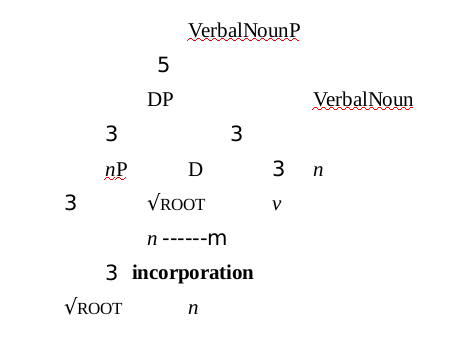
\includegraphics[height=.3\textheight]{figures/japanesetree.png}
% % % \todo[inline]{tree will be redrawn properly}
\z \z

I assume that roots are categorially neutral and a functional head like \textit{n} or \textit{v} categorizes the root (cf. \citealt{Marantz1997}). \textit{n} and \textit{v} form phases, in whose complement the semantics is fixed (cf. \citealt{Embick2010}). Therefore, (\ref{ex:nishiyama:30}a), the structure for (\ref{ex:nishiyama:29}a), can have a specialized meaning.\footnote{Strictly speaking, (\ref{ex:nishiyama:30}a) is a structure for a dvandva like \textit{oya-ko} ‘parent-child,’ and the compounds in (\ref{ex:nishiyama:12}a) and (\ref{ex:nishiyama:29}a) have a more articulated structure as proposed by \citet[83f]{ItoMester2003}. But I abstract away from this issue and (over)simplify the structure.} In contrast, in (\ref{ex:nishiyama:30}b), the structure for (\ref{ex:nishiyama:29}b), the meaning of \textit{katee} is fixed by \textit{n} before \isi{incorporation}. Therefore, subsequent \isi{incorporation} has no semantic effect and (\ref{ex:nishiyama:29}b) has a compositional meaning. In (\ref{ex:nishiyama:30}b), only the categorized root is incorporated. Therefore, any other parts of the DP (if there are any) are stranded. This is what we observed in \REF{ex:nishiyama:3}, \REF{ex:nishiyama:14}, \REF{ex:nishiyama:19}, and \REF{ex:nishiyama:28}.

One implication of the above analysis is that real compounds like \textit{yooroppa-ryokoo} ‘Europe-traveling’ (\ref{ex:nishiyama:12}a) and \textit{katee-hoomon} ‘home-visiting’ (\ref{ex:nishiyama:29}a), although they look like synthetic compounds like \textit{mountain climbing}, do \textit{not} involve noun \isi{incorporation}. In other words, despite appearances, there is no thematic relation between the right-hand element (apparent predicate) and the left-hand element (apparent argument) in (\ref{ex:nishiyama:12}a) and (\ref{ex:nishiyama:29}a). In this sense, there is no structural difference between \textit{yooroppa-ryokoo} ‘Europe-traveling’ and \textit{yooroppa-rengoo} ‘the European Union,’ and referring to the former as a \isi{synthetic compound} is in fact a misnomer. Any relationship in these compounds is established based on our world knowledge after the structure in (\ref{ex:nishiyama:30}a) is constructed.

Unlike (\ref{ex:nishiyama:12}c) and (\ref{ex:nishiyama:29}b), when noun-\isi{incorporation} involves a \isi{verbal noun} of native origin, the resulting compound has \isi{word accent}. Therefore, one cannot tell whether the structure is (\ref{ex:nishiyama:30}a) or (\ref{ex:nishiyama:30}b). The only way to tell is whether there is \isi{modifier} \isi{stranding}. Thus, when there is \isi{modifier} \isi{stranding}, we can safely say that the structure is (\ref{ex:nishiyama:30}b), involving noun \isi{incorporation}. However, without \isi{modifier} \isi{stranding} (like \REF{ex:nishiyama:18}), a compound with a \isi{verbal noun} of native origin is simply ambiguous between (\ref{ex:nishiyama:30}a) and (\ref{ex:nishiyama:30}b). \citet{Wiese2008} takes a similar position regarding synthetic compounds in \ili{German}. What is important from a cross-linguistic point of view is that, when a \ili{Sino-Japanese} \isi{verbal noun} is involved, we can differentiate the two kinds of compounds, namely word-accented compounds and phrasal-accented compounds. Given that all the phrasal-accented compounds discussed in §3.1—compounds with a \ili{Sino-Japanese} \isi{verbal noun} with a temporal \isi{suffix} attached—have a thematic relation, while many of the word-accented compounds (like \textit{doitu-bungaku} LHH-HLLL ‘\ili{German} literature’) do not, \isi{accentuation} can be a diagnostic when the analysis can be ambivalent (as in the case involving \textit{yooroppa} ‘Europe’ and \textit{ryokoo} ‘traveling’ in (\ref{ex:nishiyama:12}) that tells us whether there is a thematic relation within a compound (as (\ref{ex:nishiyama:12}c)) with the structure of (\ref{ex:nishiyama:30}b)) or not (as (\ref{ex:nishiyama:12}a) with the structure of (\ref{ex:nishiyama:30}a)).

Although I remain agnostic about whether the Baker-style \isi{incorporation} is involved for the compounding in question (cf. note 9), there is one piece of evidence for this approach. Consider the following example:

\ea\label{ex:nishiyama:31}
\gll {\ob}(*osanai) te]-dukuri\\
      {\db}{\db}{\db}childish hand-making  \\
\glt ‘(*children’s) hand-made’           \citep[220]{Sugioka2005}
\z

\textit{te-dukuri} ‘hand-made’ itself is well-formed, but it cannot have a stranded \isi{modifier}. This is a case where an adjunct (the instrumental) constitutes the left-hand element of a compound. Given that only arguments can undergo (the Baker-style) noun \isi{incorporation}, it is expected that a compound containing an instrument cannot have the structure in (\ref{ex:nishiyama:30}b); it must have the structure in (\ref{ex:nishiyama:30}a). Since only the structure in (\ref{ex:nishiyama:30}b) allows \isi{modifier} \isi{stranding}, it is expected that \textit{te-dukuri} ‘hand-made’ does not allow \isi{modifier} \isi{stranding}, which is the case, as in \REF{ex:nishiyama:31}.\footnote{For this kind of argument, it is immaterial whether the \isi{modifier} \textit{osanai} ‘childish’ is structurally an adjunct or a specifier. It is the adjunct (instrumental) status of \textit{te} ‘hand’ that is crucial.}

Admittedly, there is a pragmatic condition (i.e., being a cliché) for \isi{modifier} \isi{stranding} as discussed in the previous subsection, and \REF{ex:nishiyama:31} might be ruled out by that condition. But \isi{modifier} \isi{stranding} is systematically not observed with instrumental compounds. For example, another case of an instrumental compound is \textit{enpitu-gaki} ‘pencil-written, written with a pencil’, but this also does not allow \isi{modifier} \isi{stranding}. This is expected if the Baker-style \isi{incorporation} is involved.

Phases are assumed to be where not only semantics but also phonology is fixed. However, the structure in (\ref{ex:nishiyama:30}b) results in either \isi{word accent} or \isi{phrasal accent}, depending on whether the right-hand element is ‘heavy’ (i.e., \isi{right-branching} or \ili{Sino-Japanese}) or not. Besides, consider:

\ea\label{ex:nishiyama:32}
 \ea  tàne ‘seed’ (accent on the first mora)

  \ex
\gll {\ob}asàgao-no       tanè]-maki \\
morning.glory-\textsc{gen} {seed sowing}\\
\glt ‘sowing seeds of morning glory’\\
\glend (accent on the second mora of \textit{tane})  = (\ref{ex:nishiyama:19}b)\\
\z \z

\textit{tàne} ‘seed’ has accent on the first mora by itself (\ref{ex:nishiyama:32}a). But when incorporated, accent is on the second mora (\ref{ex:nishiyama:32}b). This suggests that \isi{accentuation} and \isi{incorporation} go hand in hand, both applying after \isi{syntax} at PF. Specifically, if we assume that accent in \ili{Japanese} is not inherently specified for each word, but that \isi{accentuation} applies to the structure obtained after all the morphological derivations are complete (cf. \citealt{Kubozono2008};\citealt{Nishiyama2010}),\footnote{In (\ref{ex:nishiyama:4}c), I introduced the traditional view that the position of accent is specified for each noun in \ili{Japanese} for expository purposes. In Kubozono's \citeyear{Kubozono2008} alternative view, nouns in \ili{Japanese} are accentuated by the default antepenultimate accent rule, and nouns whose accent is not antepenultimate (including unaccented nouns) are lexically specified as such. Such specifications and the default rule are realized after all the morphological derivations are complete. For accent in verbs in \ili{Japanese}, see \citet{Nishiyama2010}.} there is no accent shift from (\ref{ex:nishiyama:32}a) to (\ref{ex:nishiyama:32}b). In (\ref{ex:nishiyama:32}b), \textit{tane} receives accent on the second mora after compounding. In this sense, S\&K’s terminology ‘\textit{post}{}-syntactic compounds’ seems really appropriate (although their original analysis is restricted to cases involving a \ili{Sino-Japanese} \isi{verbal noun}). Also, this analysis lends support to Chomsky’s (2001) \citeyear{Chomsky2001} conjecture that head movement is not part of narrow \isi{syntax}.

\section{Phrasal compounds without noun incorporation}\label{sec:nishiyama:4}
   

As we saw in \REF{ex:nishiyama:26}, there are examples of phrasal compounds whose right-hand element is not a predicate, i.e., phrasal compounding without noun \isi{incorporation}. This section presents three other types of phrasal compounding without noun \isi{incorporation}, namely natural coordination (§4.1), suffixes/enclitics (§4.2), and prefixes/proclitics (§4.3).

\subsection{Natural coordination}\label{sec:nishiyama:4.1}
    

The following examples contain coordination as the “phrasal” part of phrasal compounds:

\ea\label{ex:nishiyama:33}
 \ea
\glll   LHHHH  LHH-HLLL\\
{\ob}karaoke to geemu]-taikai\\
{\ob}karaoke and game] contest\\  
\glt `contest for taikai' \citep[518]{Kageyama2009}\\
 \ex    
\glll HL L  LHH-HHHLLL\\
{\ob}bizyo to yazyuu]-syookoogun\\
{\ob}beauty and beast]-syndrome\\
\glt (used in a blog as synonymous to the Stockholm Syndrome)\\
\z \z

Specifically, the examples in \REF{ex:nishiyama:33} involve ‘co-compounds’ or ‘natural coordination’ forming a conceptual unit (e.g., \textit{father-mother} denoting parents, cf. \citealt{Wälchli2005}), again a kind of cliché. This usage of co-compound extends the original terminology (a.k.a. dvandva), which does not contain an overt conjunction.

By considering contrasts in \isi{accentuation}, we can confirm that in (\ref{ex:nishiyama:33}a), \textit{[karaoke to geemu]} is a phrase and \textit{geemu-taikai} is a compound. The contour of \textit{[karaoke to geemu]} is LHHHH  LHH, with two \isi{rising pitch} accents, which is typical for phrases. The word \textit{taikai} ‘content’ is inherently unaccented (LHHH), but \textit{geemu-taikai} has the contour LHH-HLLL, showing that the accent falls on the first mora of \textit{taikai}. As we saw in §2, this behavior is typical of compound \isi{accentuation}.

As we saw in \REF{ex:nishiyama:9} (repeated below), \isi{right-branching} compounds, which have \isi{phrasal accent}, do not allow a coordinate phrase as the left-hand element:

\ea%9 

   \gll *doitu to huransu    :  bungaku-kyookai\\
    Germany and France   ~ {literature association}\\
\glt    ‘associations of literature in Germany and France’
    \z

\REF{ex:nishiyama:9}         was cited in §2 to show that \isi{right-branching} compounds, despite having \isi{phrasal accent}, are not phrases but words. Since the coordinated phrase in \REF{ex:nishiyama:9} is not a natural coordination, \REF{ex:nishiyama:9} cannot be ruled in as a phrasal compound.

\subsection{Suffixes (enclitics)}\label{sec:nishiyama:4.2}
   

In the following examples, a bound morpheme attaches to a phrase:

\ea\label{ex:nishiyama:34}
 \ea        
\glll \hfill{}   LHH-HH\\
    {[}dai-kigyoo-no    syatyoo]-\textbf{kyuu}  \\
     big-company-\textsc{gen} {president equivalent}\\
\glt ‘equivalent to the president of a big company’    \citep[327]{Kageyama1993}

  \ex
\glll \hfill{}        LH-HLL\\
    {[}sakunen-no   ziko]-\textbf{irai}\\
     last.year-\textsc{gen} accident since\\
\glt ‘since last year’s accident’            (cf. \citealt[131]{Kubozono1995})

  \ex         
\glll \hfill{} {} LH-HH\\
{[}atama-ga ookii hito]-\textbf{yoo}\\
 head-\textsc{nom} big people use\\
\glt ‘for the use by big-headed people’
\z \z

Accent is specified in the last part to show that the sequence consisting of the host + -\textit{kyuu}/-\textit{irai}/-\textit{yoo} has \isi{word accent}, and therefore that the latter morphemes are integrated as part of the word. One can say that -\textit{kyuu}, -\textit{irai}, and -\textit{yoo} are suffixes, but they may better be analyzed as clitics, which are often characterized as phrasal affixes. If so, \REF{ex:nishiyama:34} involve cliticization rather than compounding. The choice of terminology is immaterial here.

The enclitics in question are originally \ili{Sino-Japanese} bound roots which have turned into clitics. As expected, there are also proclitics which originate from \ili{Sino-Japanese} bound roots; those are discussed in the next section.

\subsection{Prefixes (proclitics)}\label{sec:nishiyama:4.3}
  

Previous studies of the morphemes discussed in this subsection \citep{Poser1990,Kageyama2001,Kageyama2009} have referred to them as prefixes. However, based on the criterion mentioned in the previous subsection, namely that these morphemes attach to an entire phrase, it is preferable to call them proclitics. They are illustrated by the following examples:

\ea\label{ex:nishiyama:35}
 \ea 
\glll HL {} LHH-HLLL   \\
zen : {gaimu daizin} \\
ex {} {foreign minister}\\
\ex  
\glll HL {} LHHH \\
han : taisei\\
anti {} establishment\\
\z \z

Note that the examples have \isi{phrasal accent}. Other proclitics with this property include \textit{hòn}{}- ‘this,’ \textit{mòto}{}- ‘former,’ \textit{gèn}{}- ‘current,’ \textit{kàku}{}- ‘each,’ \textit{bòo}{}- ‘a certain,’ \textit{dòo}{}- ‘above-mentioned,’ \textit{ryòo}{}- ‘both,’ \textit{ko}{}- ‘deceased,’ \textit{hi}{}- ‘non.’

The proclitics can attach to coordinate structures, revealing their phrasal nature:

\ea\label{ex:nishiyama:36}
 \ea 
\gll {} {} LHHHLL {} LHLLL\\
ko : [Hasegawa-si to Uemura-si]      \\
late {} Hasegawa-mr and Uemura-mr \\
\glt `the late Mr. Hasegawa and Mr. Uemura'  (adapted from \citealt[265]{Kageyama2001})
\ex  
\glll {} {} LHH  H  LHHH\\
gen : [syusyoo to gaisyoo]\\
current {} prime.minister and foreign.minister\\ 
\glt ‘current prime minister and foreign minister’
\z \z

As in \REF{ex:nishiyama:33}, accent reveals the phrasal nature of the \isi{coordinate structure}.

In addition, the inherently anaphoric \isi{proclitic} \textit{dòo}{}- ‘above-mentioned’ violates the anaphoric island constraint, again strongly suggesting its phrasal status:

\ea\label{ex:nishiyama:37}
 \gll daitooryoo-wa asu     yuukoo-zyooyaku-ni tyooinsuru     doo: zyooyaku: saisyuu-an niyoruto\\
  president-\textsc{top}  tomorrow amenity-treaty-\textsc{dat}  sign       said treaty    final-version according.to\\ 
\glt ‘The President is going to sign the amenity treaty tomorrow. According to the final version of the said treaty,…’            \citep[258]{Kageyama2001}
\z

Here, \textit{doo}{}- in the second sentence refers to \textit{yuukoo} ‘amenity’ of \textit{yuukoo-zyoo\-yaku} ‘amenity treaty’. \textit{doo}{}- itself is also a part of the compound \textit{[doo: zyooyaku: saisyuu-an]}. In other words, both the anaphor and the antecedent are a part of a word, violating the anaphoric island constraint, which says that anaphoric relations cannot be established within a word.

While natural coordination in \REF{ex:nishiyama:33} and enclitics in \REF{ex:nishiyama:34} result in \isi{word accent}, proclitics in \REF{ex:nishiyama:35} and \REF{ex:nishiyama:36} result in \isi{phrasal accent}. Again this may be related to the fact that proclitics tend to yield a \isi{right-branching} structure (cf. \REF{ex:nishiyama:10}). Even with a binary structure as in (\ref{ex:nishiyama:35}b), the clitic status of the left-hand element makes the right-hand element relatively heavy, and this might induce the reanalysis of the right-hand element as bimorphemic, as with the case of noun-incorporated compounds with \ili{Sino-Japanese} predicates discussed in \REF{ex:nishiyama:23}.

\section{Reconsidering “Word Plus”}\label{sec:nishiyama:5}
\citet{Kageyama1993,Kageyama2001,Kageyama2009} proposes the new term \isi{Word Plus}, which covers all the phrasal-accented compounds minus what he and S\&K term post-syntactic compounds as discussed in \sectref{sec:nishiyama:3.1}. The level of \isi{Word Plus} comes between a word and a phrase, and this is meant to capture the dual (i.e., word and phrasal) nature of the examples in question.

In my view, the notion \isi{Word Plus} subsumes heterogeneous examples. First of all, many instances of Kageyama’s \isi{Word Plus} are \isi{right-branching} compounds of the type in (\ref{ex:nishiyama:8}b), which cannot be analyzed as involving a phrase, as we saw in \REF{ex:nishiyama:9}. This leaves us with prefixes (discussed in §4.3) and non-\isi{right-branching} pseudo compounds. Let us discuss them in turn.

We saw in §4.3 that the proclitics in question have phrasal nature, in that they can attach to a phrase. But Kageyama argues that they have a word-like nature as well. The evidence comes from ellipsis:

\ea\label{ex:nishiyama:38}
\gll  *A-wa gen :   \st{kaityoo-to}    \st{suruai-de},    B-wa zen : kaityoo-to    siriai-da\\
  A-\textsc{top} current ~ president-with acquainted-\textsc{cop}  B-\textsc{top} ex ~ president-with  acquainted-\textsc{cop}\\
\glt  ‘A \st{is acquainted with the current president}, and B is acquainted with the ex-president.’
\citep[251]{Kageyama2001}
\z

The strikethrough indicates (cataphoric) ellipsis under identity. If \textit{gen} is replaced with \textit{genzai-no} ‘current-\textsc{gen}’ and \textit{zen} is replaced with \textit{mae-no} ‘former-\textsc{gen}’, the sentence becomes \isi{grammatical}. On the assumption that ellipsis is possible with phrases, Kageyama argues that \REF{ex:nishiyama:38} is evidence for the word-like nature of the proclitics in question.

However, \REF{ex:nishiyama:38} is independently ruled out, because a clitic \textit{gen=}{}- -- a bound morpheme -- does not have a host after ellipsis. Alternatively, \REF{ex:nishiyama:38} is accounted for by assuming that the presence of the \isi{genitive} is required for recovering the elided part. This is analogous to the following contrast in \ili{English}:

\ea\label{ex:nishiyama:39}
 \ea[]{John’s dog is bigger than Bill’s \st{dog}.}
 \ex[*]{John’s dog is bigger than Bill\st{’s dog}.}
\z \z

\citet{Lobeck1990} proposes an analysis of ellipsis based on Spec-Head agreement, but regardless of the validity of this analysis, whatever account captures the contrast in \REF{ex:nishiyama:39} would also account for \REF{ex:nishiyama:38}.

  Another piece of evidence that Kageyama cites for his observation that the proclitics in question are word-level (as opposed to phrasal level) entities is the following:

\ea\label{ex:nishiyama:40}
 \ea 
\gll  yuumee-na     haiyuu   \\
    famous-\textsc{mod}    actor\\

 \ex
\gll   ??yuumee-hàiyuu\\
        {\db}{\db}famous-actor\\
  \ex
\gll  tihòo-no     tòsi   \\ 
    province-\textsc{gen} city   \\

  \ex
\gll   tihoo-tòsi\\
     province-city\\
\z \z

\ea\label{ex:nishiyama:41}
 \ea  
\gll bòo : [yuumee (*na) haiyuu]\\
    certain ~ famous \textsc{mod} actor\\
\glt ‘a certain famous actor’

  \ex 
\gll  kàku : [tihoo (*no) tòsi] \\
    each ~ province \textsc{gen} city\\
\glt ‘each provincial city’      (\citealt[249f]{Kageyama2001})
\z \z

\textit{yuumee-na haiyuu} ‘famous actor’ (\ref{ex:nishiyama:40}a) and \textit{tihòo-no tòsi} ‘provincial city’ (\ref{ex:nishiyama:40}c) are phrases, and the former cannot be a compound (\ref{ex:nishiyama:40}b), but the latter can (\ref{ex:nishiyama:40}d). The examples in \REF{ex:nishiyama:41} illustrate cases with proclitics, and the \isi{modifier} \isi{marker} \textit{na} and the \isi{genitive} \isi{marker} \textit{no} cannot appear here. This means that the prolicitcs cannot attach to a phrase (with \textit{na} or \textit{no}) but must attach to a word (i.e. here, to a compound). The contrast between (\ref{ex:nishiyama:40}b) and (\ref{ex:nishiyama:41}a) is telling: the compound \textit{??yuumee-hàiyuu} does not exist by itself, but with the \isi{proclitic} \textit{bòo}{}-, the compound must be used. If \textit{bòo}{}- and \textit{kàku}{}- are clitics, they should be able to attach to a full phrase, and (\ref{ex:nishiyama:41}) should be possible with \textit{na/no}, contrary to fact. This, according to Kageyama, is evidence for the word-like nature of the proclitics in question.

The above point is well taken, but cross-linguistically, the distinction between clitics and affixes is often not categorial but a matter of degree. For example, \ili{Romance} clitics are often analyzed as being on a grammaticalization path towards agreement markers (namely suffixes) (cf. \citealt{Suner1988}, among others). Thus, the hybrid nature of the morphemes in question might simply reflect the hybrid nature of clitics in general, and this alone is not sufficient as a motivation for postulating a novel level of \isi{Word Plus}.

Non-\isi{right-branching} pseudo compounds are of two types: binary compounds with \isi{phrasal accent} and \isi{left-branching} compounds with \isi{phrasal accent}. The former is illustrated by the following example:

\ea\label{ex:nishiyama:42}
\gll   kyùusyuu : nànbu\\
    Kyuusyuu ~ southern.part\\
\glt ‘Southern Kyusuyu’    (\citealt[70]{Kubozono1995}, also cited in \citealt[261]{Kageyama2001})
\z

We have been assuming that (exceptional) \isi{phrasal accent} in compounds is due to a \isi{right-branching} structure. So why does \REF{ex:nishiyama:42} have \isi{phrasal accent}, unlike ordinary compounds (with \isi{word accent}), although it is not \isi{right-branching}?

One important point is that \REF{ex:nishiyama:42} optionally can have the \isi{genitive} between the two parts of the construction, and when this happens, we have \isi{phrasal accent}, as expected:\footnote{\citet[70]{Kubozono1995} notes that person names also have \isi{phrasal accent}. Here as well, the \isi{genitive} \isi{marker} used to appear between the family name and the given name; however, this usage of the \isi{genitive} \isi{marker} has become obsolete.} 

\ea\label{ex:nishiyama:43}
\gll   kyùusyuu-no  nànbu\\
    Kyuusyuu-\textsc{gen} southern.part\\
\glt ‘southern part of Kyuusuyuu’
\z

It is reasonable to analyze \REF{ex:nishiyama:42} as involving \isi{genitive} deletion. Therefore, \REF{ex:nishiyama:42} is not a compound in a strict sense, but is better called a phrase in disguise.

Since the \isi{genitive} usually cannot be left out, I conjecture that it is the \textit{cliché} nature of \REF{ex:nishiyama:42} that makes \isi{genitive} deletion possible. Thus, Kyuusyuu is an island stretching from north to south, and is usually referred to as having a northern and a southern part.\footnote{Kubozono’s (1995: 71f) account is couched in terms of “semantic unity.” Regarding this, \citet[261]{Kageyama2001} states that “it is difficult to delimit the range of phrase-like [pseudo] compounds in term of their internal semantic relations.” In the context of the current discussion, Kubozono’s insight is reinterpreted as a pragmatic factor leading to cliché.  It should also be noted that the examples in \REF{ex:nishiyama:42} and \REF{ex:nishiyama:43} are different from \textit{haha no hi} ‘Mother’s Day’ and \textit{ama no zyaku} ‘devil’s advocate’, which do not allow \isi{genitive} deletion. \citet[268]{Kageyama2001} cites them as \ili{Japanese} equivalents of \isi{possessive} compounds (e.g., \textit{a girls’ school}), and says that “those expressions are completely lexicalized.” This is corroborated by the fact that they have \isi{word accent}, as opposed to \REF{ex:nishiyama:42} and \REF{ex:nishiyama:43}, which have \isi{phrasal accent}.}

  A similar deletion process is involved with -\textit{teki} (repeated):


\begin{exe}%2
%     \label{ex:nishiyama:2}

    %\ex  
\exi{(2)}
    \gll dare-ga    bosu-da-teki      tàido\\
    who-\textsc{nom}  boss-\textsc{cop}-like  attitude\\
\glt ‘a who’s the boss attitude’
    \z

\textit{teki}{}- usually attaches to a root and derives an \isi{adjectival} noun, which requires \textit{na} as the modifying \isi{marker} as in (\ref{ex:nishiyama:44}a):

\ea\label{ex:nishiyama:44}
 \ea  
\gll hankoo-teki-na     tàido\\
    rebellion-like-\textsc{mod}  attitude\\
\glt ‘rebellious attitude’
 
 \ex
\gll   hankoo-teki :  tàido\\
    rebellion-like  ~ attitude\\

\glt ‘rebellious attitude’
\z \z

But as (\ref{ex:nishiyama:44}b) shows, the modifying \isi{marker} \textit{na} can be left out, resulting in what looks like a pseudo compound (with \isi{phrasal accent}). In (\ref{ex:nishiyama:2}b) as well, \textit{na} can emerge after -\textit{teki}. The alternation between (\ref{ex:nishiyama:44}a) and (\ref{ex:nishiyama:44}b) is analogous to the presence and absence of \textit{no} in \REF{ex:nishiyama:43} and \REF{ex:nishiyama:42}.

  Apparent \isi{left-branching} pseudo compounds are illustrated as follows:

\ea\label{ex:nishiyama:45}
 \ea
\gll  booeki-gàisya : syatyoo\\
    trading-company ~ president\\

  \ex
\gll  siritu-dàigaku : kyoozhu\\
    private-university ~ professor    (\citealt[518f]{Kageyama2009})\\
\z \z

The \isi{genitive} deletion analysis proposed above for binary pseudo compounds can be extended to this case. These examples are also fixed expressions; they refer to some distinguished titles, and \textit{syatyoo} ‘president’ cannot be replaced by \textit{sarariiman} `salaried worker’ and \textit{kyoozyu} ‘professor’ cannot be replaced by \textit{syokuin} ‘worker’ in this kind of expression.

To summarize, Kageyama’s notion of \isi{Word Plus} is not a natural class and should be reclassified into three distinct classes: \isi{right-branching} compounds, constructions involving proclitics, and phrases involving \isi{genitive} deletion.

The genitive-deletion analysis is actually suggested by \citet[163, n. 7]{KageyamaShibatani1989} for \isi{right-branching} pseudo compounds as in (\ref{ex:nishiyama:8}b). However, as we saw in \REF{ex:nishiyama:9}, the \isi{right-branching} pseudo compounds of the type in (\ref{ex:nishiyama:8}b) cannot contain a phrase. Therefore, it is unlikely that they involve \isi{genitive} deletion.

In fact, in later works Kageyama (\citeyear{Kageyama1993}: 342, \citeyear{Kageyama2001,Kageyama2009}) does not endorse his own earlier suggestion of \isi{genitive} deletion mentioned above and develops the \isi{Word Plus} analysis instead. In particular, he notes (\citeyear{Kageyama2001}:250f, \citet{Kageyama2009}:519) notes that partial ellipsis is impossible with pseudo compounds, although it is possible when the \isi{genitive} is present.

\ea\label{ex:nishiyama:46}
 \gll A-wa siritu-daigaku  *(no) \st{kyoozyu-de},  B-wa kokuritu-daigaku *(no) kyoozyu desu\\
  A-\textsc{top} private-university \textsc{gen} {professor \textsc{cop}}  B-\textsc{top} national-university \textsc{gen} professor \textsc{cop}\\
\glt   ‘A \st{is a professor} (of) a private university, and B is a professor of a national university.’
(adapted from \citealt[519]{Kageyama2009})
\z

This might be taken as evidence against the genitive-deletion analysis. However, as mentioned after \REF{ex:nishiyama:38}, the contrast in question is accounted for by assuming that the presence of the \isi{genitive} is required for recovering the elided part. Thus, the ungrammaticality of \REF{ex:nishiyama:46} without \textit{no} is not an obstacle for postulating \isi{genitive} deletion for deriving \isi{left-branching} pseudo compounds as in \REF{ex:nishiyama:45}.

\section{Conclusions}\label{sec:nishiyama:6}

This paper has discussed phrasal compounds in \ili{Japanese}, reanalyzing and reclassifying examples discussed in the previous studies in this area. One important mechanism for phrasal compounding is noun \isi{incorporation}, although I leave open the exact mechanism of this process. I have extended \citegen{ShibataniKageyama1988} and \citegen{KageyamaShibatani1989} analysis of post-syntactic compounds (involving \ili{Sino-Japanese} \isi{verbal noun}) to verbal nouns of native origin. A noun-\isi{incorporation} analysis for compounds involving verbal nouns of native origin has been proposed by \citet{Sugioka2002}, but I have refined the analysis. Specifically, compounds involving verbal nouns of native origin are structurally ambiguous, with one structure involving noun \isi{incorporation} and the other without noun \isi{incorporation}. Only when there is \isi{modifier} \isi{stranding} can we be certain that noun \isi{incorporation} is involved.

Through the classification of phrasal compounds, I have claimed that Kageyama’s (\citeyear{Kageyama1993,Kageyama2001,Kageyama2009}) notion of \isi{Word Plus} should be reclassified into three existing types, namely \isi{right-branching} compounds, constructions involving proclitics, and phrases involving \isi{genitive} deletion.

Here is a table summarizing the proposed analyses and classes of phrasal compounds in \ili{Japanese}:

\begin{table} 
\small
\begin{tabularx}{\textwidth}{QQQ}
\lsptoprule
\multicolumn{3}{l}{ noun incorporation}\\
 Sino- \ili{Japanese}\newline  \isi{verbal noun} & \multicolumn{2}{l}{ \isi{verbal noun} of native origin} \\
\midrule
\textit{yooròppa : ryokoo} 
\newline 
‘Europe traveling’ (\ref{ex:nishiyama:12}c) & {{\itshape asagao-no       tane-maki}
\newline 
‘sowing seeds of morning glory’ (\ref{ex:nishiyama:19}b)} & \textit{kireena mati-dukuri}
\newline 
 ‘construction of a clean town’
\REF{ex:nishiyama:3}\\
& \multicolumn{1}{l}{relational noun} & cliché \\ 
\end{tabularx}

% \medskip

\begin{tabularx}{\textwidth}{QQQQ} 
\midrule
 \multicolumn{4}{l}{ NO noun incorporation}\\
modifying structure & \isi{coordinate structure} & prefix/\newline \isi{proclitic} & \isi{suffix}/\newline \isi{enclitic}\\
\midrule
 {\itshape tiisana sinsetu-undoo}
\newline 
 ‘campaign for doing small kindness’ (\ref{ex:nishiyama:26}a) & 
\textit{bizyo to yazyuu-syookoogun}
\newline 
 `beauty and beast-syndrome' (\ref{ex:nishiyama:33}b) & 
\textit{dai-kigyoo-no    syatyoo-kyuu}
\newline 
 ‘equivalent to the president of a big company’
(\ref{ex:nishiyama:34}a) & 
{\itshape zèn : gaimu-dàizin}
\newline 
 ‘ex-foreign minister’
(\ref{ex:nishiyama:35}a)\\
cliché & cliché &  & \\
\lspbottomrule
\end{tabularx}


\caption{Summary and representative examples of types of phrasal compounds in Japanese}
\end{table} 


Phrasal compounds are classified primarily by whether noun \isi{incorporation} is involved or not. If it is, a further division is made according to whether the predicate is of \ili{Sino-Japanese} or of native origin. With a \ili{Sino-Japanese} \isi{verbal noun}, the resulting compound has \isi{phrasal accent}. In contrast, with a \isi{verbal noun} of native origin, one cannot tell whether the compound is formed by noun \isi{incorporation} or not without \isi{modifier} \isi{stranding}. This is why the above examples have \isi{modifier} \isi{stranding}, to make the case for the phrasal status of the complement of the \isi{verbal noun}. There are two licensing conditions for \isi{modifier} \isi{stranding}: the complement of the predicate---the left-hand element of the compound---should be a \isi{relational noun} or a part of a cliché.

If no noun \isi{incorporation} is involved, there are four subclasses. With modifying structures and coordinate structures, the licensing condition is again cliché. Prefixes/proclitics and suffixes/enclitics originate in \ili{Sino-Japanese} bound roots, but they have become clitics, so that they attach to a phrase. Given the ability of clitics to attach to entire phrases, they don’t have to obey any conditions (such as cliché) in order to participate in the formation of phrasal compounds.

Lastly, I summarize and clarify my standpoint regarding the relationship between accent and \isi{syntax}. As we saw in (\ref{ex:nishiyama:8}b), \textit{dòitu : bungaku-kyòokai} ‘\ili{German} Association of Literature’ has \isi{phrasal accent}, but is not a phrasal compound. Conversely, there are cases of phrasal compounds with \isi{word accent}. \textit{kìreena mati-dùkuri} ‘construction of a clean town’ in \REF{ex:nishiyama:3} has \isi{word accent} in the \textit{mati-dùkuri} ‘city-making’ part, but it is a phrasal compound as a whole. Furthermore, \textit{yooròppa : ryokoo-tyùu} ‘while traveling in Europe’ in (\ref{ex:nishiyama:12}c) has \isi{phrasal accent} but is analyzed as a compound. These situations manifest a kind of syntax-phonology mismatch and might give an impression that accent is not a reliable diagnostic for determining whether a string is a word or a phrase.

However, I believe that the hypothesis that accent in \ili{Japanese} reflects the syntactic status is basically correct. Specifically, whenever a string [A B] has \isi{word accent}, it is always analyzed as a compound. In the case of \textit{kìreena mati-dùkuri} ‘construction of a clean town’ in \REF{ex:nishiyama:3}, the word status of the \textit{mati-dùkuri} part is independently confirmed by \textit{rendaku} sequential voicing, as we saw in \sectref{sec:nishiyama:3.2.1}. In this sense, the other two cases are exceptional, but not without a reason. \textit{dòitu : bungaku-kyòokai} ‘\ili{German} Association of Literature’ in (\ref{ex:nishiyama:8}b) has \isi{phrasal accent} because it is a \isi{right-branching} compound, which requires a special treatment for ease of processing, as we saw at the end of \sectref{sec:nishiyama:2}. For \textit{yooròppa : ryokoo-tyùu} ‘while traveling in Europe’ in (\ref{ex:nishiyama:12}c), accent is really unhelpful, but the fact that an adverb cannot intervene between the two parts shows that it is not a phrase but a word, as we saw in \REF{ex:nishiyama:13}. Its (exceptional) \isi{phrasal accent} has been attributed to the \ili{Sino-Japanese} nature of the \isi{verbal noun}.
 



\section*{Acknowledgements}
Earlier versions of this paper were presented in a meeting of the Lexicon Study Circle at Keio University and at the Workshop on Phrasal Compounds at University of Mannheim. I thank Carola Trips and Jaklin Kornfilt for inviting me to the workshop. For valuable comments and suggestions, I thank the audiences, Yoko Sugioka and Ichiro Yuhara. I also thank Jaklin Kornfilt for detailed and helpful comments on the earlier version of this paper. This study has been supported by grants from the Japan Society for the Promotion of Science (Grant \# 23520454, 15K02470).


{\sloppy
\printbibliography[heading=subbibliography,notkeyword=this]
}

\end{document}